I projektets spæde start, optegnede vi med GitHubs projekt funktion, en Sprint-plan for hele projektets periode. En Sprint, betegner en arbejdsuges/skoleuge som i vores tilfælde er mandag til fredag. Planen så således ud:

\begin{table}[H]
\centering
\renewcommand{\arraystretch}{1.4}
\begin{tabular}{>{\bfseries}l l}
    \toprule
    \rowcolor{headerblue}
    \textcolor{white}{\textbf{Periode}} & \textcolor{white}{\textbf{Opgave}} \\
    \midrule
    Uge 11 & Projektstart \\
    \rowcolor{lightgray}
    Uge 12 & Controller movement \\
    Uge 13 & Opløsning og skalering (bar) \\
    \rowcolor{lightgray}
    Uge 13 & Pixel art \\
    Uge 15 & Monsterlogik (patrol script) \\
    \rowcolor{lightgray}
    Uge 15 & Skydesystem \\
    Uge 16 & Shopsystem og meta-progression \\
    \rowcolor{lightgray}
    Uge 17 & Intensiv rapportskrivning \\
    Uge 19 & Bufferperiode \\
    \rowcolor{deadlinered}
    \textcolor{white}{Deadline 18/05} & \textcolor{white}{\textbf{Aflevering}} \\
    \rowcolor{lightgray}
    \bottomrule
\end{tabular}
\caption{Sprint Plan – DDU Teknikfagsprojekt}
\end{table}

Denne plan afspejler selvfølgelig ikke hvordan projektet forløb i virkeligheden, da ting altid tager længer tid end forventet. 
Vi har løbende måtte fortage ændringer i den plan for at tage hånd om dele som enten har været foran eller bagud for planen. Vi har måtte håndterer en hel del uforudsete udfordringer som sygdom, som har gjort at vi måtte ændre i planen. Den omplanlægning har ikke været af aller højeste kvalitet, men selvom det har projektet aligevel lykkeds. Det skyldes at gruppens størrelse ikke var størere end den er og vi har derfor kunne fortage beslutninger ad hoc som man ellers ikke normalt i større spiludviklingsprojekter ville gøre.

Planen er opstillet i en prioriteret rækkefølge med de vigtigste grundelementer, som danner grundlaget for et spilbart spil.

\todo[inline]{Angiv standup-referater og link til SCRUM}

\todo[inline]{Nævn Git}

\todo[inline]{Visualiser forgrening af GitHub-projekt}

\subsection{\LaTeX\ ToDo-notes}
Selve rapporten her er skrevet i \LaTeX-kode, læs om \LaTeX i \autoref{sec:latexsoftware}, og sidenhen kompileret via \mintinline{bash}{pdflatex}. En særlig \LaTeX-package, er \mintinline{bash}{todonotes}, der gør det muligt at oprette to-do-noter, der så inkluderes i den kompilerede pdf. Det har muliggjort planlægning af strukturen i rapporten direkte i rapporten, og således har vi ikke behøvet et separat system til at holde styr på rapportens indhold. Det betyder også, at man bliver konfronteret med noterne undervejs, og man bliver således nødt til at forholde sig til dem. To-do-noterne er også blevet brugt som et rudimentært skelet, og som færdighedsmarkør---hvor at en ToDo-note viser, at et kapitel ikke er færdigskrevet. Af \autoref{fig:todonote} fremgår, hvordan disse todonotes ser ud, når \LaTeX-dokumentet er kompileret.

\begin{figure}[H]
  \centering
  \fbox{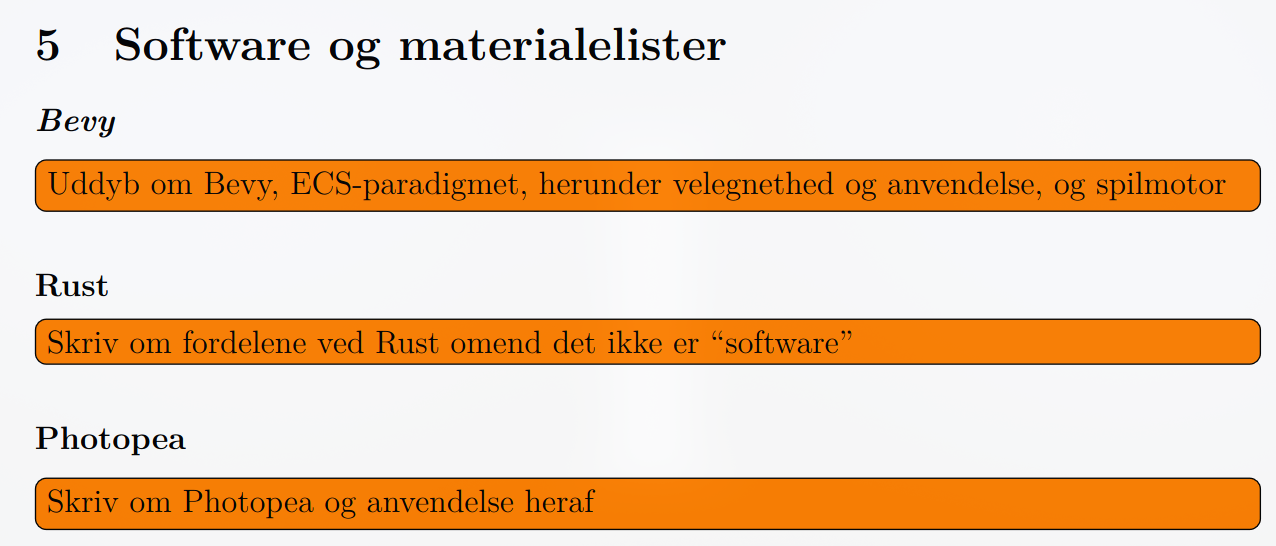
\includegraphics[width=0.85\textwidth]{assets/todoeksempel.png}}
  \caption{Viser en to-do-note fra packagen \mintinline{bash}{todonotes}. Her oprettet via \mintinline{latex}{\todo[inline]{...}} osv. Bemærk, at den er oprettet med \mintinline{latex}{inline}, da to-do-noten ellers placeres i dokumentets margen, hvilket kan se mærkeligt ud, især når indholdet i todo-noten er tilpas stor.}\label{fig:todonote}
\end{figure}
